\chapter{Game Controllers}

The \jr\ allows you to connect either Atari style joysticks or NES/SNES style gamepads as game controllers. The two different styles of controllers are used differently and are supported by different registers on the \jr. Note: Atari style analog devices are not supported ({\it e.g.} paddles, analog joysticks, analog mice).

\section*{Atari Style Joysticks}

The \jr\ has two IDC headers that can be connected to a DB-9 socket to allow Atari style joysticks to be used (see figure:~\ref{fig:joystick_ports} for the pinouts). Joystick header 0 is wired to the pins of Port B of the VIA (see page~\ref{chap_via}), and joystick header 1 is connected to Port A. The various joystick switches are connected to the ports in same manner as on the C-64, with the exception that more buttons are supported (see table:~\ref{tab:via_joystick}).

\begin{figure}[ht]
    \begin{center}
        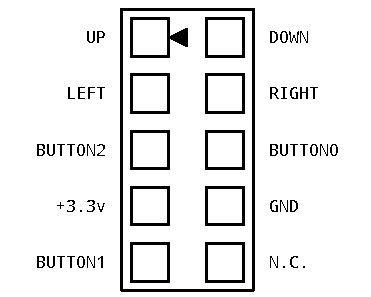
\includegraphics[scale=0.65]{images/f256_port_joystick.pdf}
    \end{center}
    \caption{Joystick Port Pinouts}
    \label{fig:joystick_ports}
\end{figure}

In order to use the joysticks, the DDR bits for the ports must be set to 0 for input. Then the input/output register for the port may be read. If a button or switch is closed on the joystick, the corresponding bit in the I/O register will be clear (0). If the button is not pressed, the bit will be set (1).

As a reminder: be aware that the WDC65C22 on the \jr\ is being used with a 3.3 volt supply. This means that any device plugged into the joystick ports should be 3.3 volt tolerant and should not raise any pin above 3.3 volts, otherwise damage could occur.

\begin{table}[ht]
    \begin{center}
        \begin{tabular}{|c|c|c|c|c|c|c|c|} \hline
            7 & 6 & 5 & 4 & 3 & 2 & 1 & 0 \\\hline\hline
            --- & BUTTON2 & BUTTON1 & BUTTON0 & RIGHT & LEFT & DOWN & UP \\ \hline
        \end{tabular}
    \end{center}
    \caption{Joystick Flags}
    \label{tab:via_joystick}
\end{table}

\example{Displaying Joystick 1}
In this example, we will poll joystick 1 and print out the state of all the buttons by printing the byte we read from the joystick port as a simple binary number. The example will try to be a little smart by only printing the value when the value has changed. NOTE: this example expects OpenKernal to be installed, and will call two of its routines for initializing the screen and printing a character.

First, we initialize the screen, the variable we use to track the old value of the joystick port, and the VIA (setting port A to be an input port):
\begin{verbatim}
ok_cint = $FF81                         ; OpenKernal: init the screen
ok_cout = $FFD2                         ; OpenKernal: print the character in A

; Variables

* = $0080

value:      .byte ?                     ; Variable for the old joystick value
prv:        .byte ?                     ; Copy of value for printing

* = $e000

start:      jsr ok_cint                 ; Set up the screen

            lda #$FF                    ; Set the previous value to $FF
            sta value

            stz MMU_IO_CTRL             ; Switch to I/O Page 0

            lda #$00                    ; Set VIA Port A to input
            sta VIA_DDRA
\end{verbatim}

Next, we print the OpenKernal code to clear the screen, and we print out the byte in \verb+value+ as a binary number.

\begin{verbatim}
loop1:      lda #147                    ; Print the CBM clear screen code
            jsr ok_cout

            lda value                   ; Copy the value to prv
            sta prv

            ldx #8                      ; Loop for all eight bits
loop2:      asl prv                     ; Shift MSB into the carry
            bcc is0                     ; If it's 0, print '0'

            lda #'1'                    ; Otherwise, print '1'
            jsr ok_cout
            bra repeat                  ; And go to the next bit

is0:        lda #'0'                    ; Print '0'
            jsr ok_cout

repeat:     dex                         ; Count down
            bne loop2                   ; Repeat until we've done all 8 bits
\end{verbatim}

Next, we read the value of port A. If it is different from \verb+value+, we save it to \verb+value+ and go back to print the byte we read. Otherwise, we keep waiting and polling the joystick port.

\begin{verbatim}
            stz MMU_IO_CTRL             ; Switch to I/O Page 0

wait:       lda VIA_IORA                ; Get the status of port A
            cmp value                   ; Is it different from before?
            beq wait                    ; Yes: keep waiting

            sta value                   ; Save this value as the previous one
            bra loop1                   ; And go to print it
\end{verbatim}

\section*{NES/SNES Gamepads}

The \jr\ also provides support for NES/SNES compatible gamepads. NES gamepads work a little differently from Atari style joysticks. Where Atari style joysticks are directly readable through the VIA ports, NES gamepads communicate to the \jr\ through a serial interface. To read the gamepad, a program needs to first send the signal to the gamepad to capture the status of all the buttons, then the program needs to trigger the system to transfer the button status over the serial interface to the computer. This transfer takes a few clock cycles, since it is done serially, so the program needs to wait until the NES registers indicate that the transfer is done.

Before any transfer is done, the program must specify (by setting or clearing the MODE bit) whether the gamepad is NES compatible or SNES compatible. NES gamepads only send 8 bits of data, but SNES controllers send 12 bits. The NES/SNES data register are arranged differently depending on the value of MODE.

The process the program follows to read the state of the gamepad is:

\begin{enumerate}
    \item Set NES\_EN of NES\_CTRL to enable the NES/SNES support (see table~\ref{tab:nes_registers}) and set or clear MODE, to choose between NES mode or SNES mode.
    \item Set NES\_TRIG of NES\_CTRL to sample the buttons and transfer the data to the registers.
    \item Read NES\_STAT and wait until the DONE bit is set
    \item Check the appropriate NES or SNES control registers (see table~\ref{tab:nes_data_reg})
    \item Clear NES\_TRIG
\end{enumerate}

\begin{table}[ht]
    \begin{center}
        \begin{tabular}{|c|c|c|c|c|c|c|c|c|c|c|} \hline
            Address & R/W & Name & 7 & 6 & 5 & 4 & 3 & 2 & 1 & 0 \\\hline\hline
            \verb+0xD880+ & W & NES\_CTRL & NES\_TRIG & \multicolumn{4}{|c|}{---} & MODE & --- & NES\_EN \\ \hline
            \verb+0xD880+ & R & NES\_STAT & NES\_TRIG & DONE & \multicolumn{3}{|c|}{---} & MODE & --- & NES\_EN \\ \hline
        \end{tabular}
    \end{center}
    \caption{NES/SNES Gamepad Registers}
    \label{tab:nes_registers}
\end{table}

\begin{description}
    \item[NES\_CTRL] Set (1) to start the process of sampling the buttons.
    \item[DONE] If set (1), the gamepad status has been read into the registers, and is available for reading
    \item[MODE] If set (1), the gamepad is expected to be an SNES compatible controller. If clear (0), the gamepad is expected to be an NES compatible controller.
    \item[NES\_EN] If set (1), enables NES/SNES controller support.
\end{description}

\begin{table}[ht]
    \begin{center}
        \begin{tabular}{|c|c|c|c|c|c|c|c|c|c|c|} \hline
            MODE & Address & Pad & 7 & 6 & 5 & 4 & 3 & 2 & 1 & 0 \\\hline\hline
            \multirow{4}{*}{0} & 0xD884 & 0 & A & B & SELECT & START & UP & DOWN & LEFT & RIGHT \\\cline{2-11}
                & 0xD886 & 1 & A & B & SELECT & START & UP & DOWN & LEFT & RIGHT \\\cline{2-11}
                & 0xD888 & 2 & A & B & SELECT & START & UP & DOWN & LEFT & RIGHT \\\cline{2-11}
                & 0xD88A & 3 & A & B & SELECT & START & UP & DOWN & LEFT & RIGHT \\\hline\hline

            \multirow{8}{*}{1} & 0xD884 & \multirow{2}{*}{0} & B & Y & SELECT & START & UP & DOWN & LEFT & RIGHT \\\cline{2-2}\cline{4-11}
                               & 0xD885 &                    & \multicolumn{4}{|c|}{---} & A & X & L & R \\\cline{2-11}
                               & 0xD886 & \multirow{2}{*}{1} & B & Y & SELECT & START & UP & DOWN & LEFT & RIGHT \\\cline{2-2}\cline{4-11}
                               & 0xD887 &                    & \multicolumn{4}{|c|}{---} & A & X & L & R \\\cline{2-11}
                               & 0xD888 & \multirow{2}{*}{2} & B & Y & SELECT & START & UP & DOWN & LEFT & RIGHT \\\cline{2-2}\cline{4-11}
                               & 0xD889 &                    & \multicolumn{4}{|c|}{---} & A & X & L & R \\\cline{2-11}
                               & 0xD88A & \multirow{2}{*}{3} & B & Y & SELECT & START & UP & DOWN & LEFT & RIGHT \\\cline{2-2}\cline{4-11}
                               & 0xD88B &                    & \multicolumn{4}{|c|}{---} & A & X & L & R \\\hline
        \end{tabular}
    \end{center}
    \caption{NES/SNES Data Registers}
    \label{tab:nes_data_reg}
\end{table}

NOTE: If you want to use NES/SNES controllers with the \jr, you will need to add an adapter to convert the common port to NES and SNES connectors. The Foenix shop has the adapter, which comes in one of two flavors: one for the \jr\ (which has an IDC pin header on the board for the NES/SNES controollers), and one for the F256k (which has a 9 pin mini-DIN connector on the back).